% !TEX root = ../seapp-manual.tex

% Chapter 3 - Set up and run a new SEA++ scenario

\chapter{Set up and run a new SEA++ scenario}
\label{ch:run-scenario}

SEA++ is distributed with a complete set of examples that are ready to use. However, the process to build a new SEA++ scenario is substantially identical to that of INET.

\section{Traditional Networks}

In the following example is shown how to set up a new simple scenario in which there are a client and a server.

\paragraph{\nth{1} step - make the folder}
As in INET, the \nth{1} step is to make the folder that will contain all the new files, e.g. scenario.
%
\begin{lstlisting}[language={terminal}]
@~/seapp_stable/inet/examples/@ mkdir scenario
@~/seapp_stable/inet/examples/@ cd scenario
\end{lstlisting}


\paragraph{\nth{2} step - network description}
As in INET, the \nth{2} step is to edit the \texttt{.ned} file that contains the network description, e.g. \texttt{scenario.ned}.
%
\begin{lstlisting}[language={ned}, caption={scenario.ned}, label={lst:build-scenario-ned}]
package inet.examples.inet.scenario;

import inet.networklayer.autorouting.ipv4.IPv4NetworkConfigurator;
import inet.nodes.inet.StandardHost;
import inet.globalfilter.GlobalFilter;

network scenario
{
  parameters:
    string attackConfigurationFile = default("none");
    double n;

  submodules:
    globalFilter: GlobalFilter;
    client: StandardHost;
    server: StandardHost;
    configurator: IPv4NetworkConfigurator;
        
  connections allowunconnected:
    client.pppg++ <--> { datarate = 10Mbps; } <--> server.pppg++;
    globalFilter.nodes++ <--> client.global_filter;
    globalFilter.nodes++ <--> server.global_filter;
    
}
\end{lstlisting}

In this step, is fundamental to:
%
\begin{itemize}
\item add the the string parameter \texttt{attackConfigurationFile} to the network;
\item import the GlobalFilter class, declare a GlobalFilter submodule and connect it to all the other nodes.
\end{itemize}

In case of \textbf{disable} primitive it is necessary to import and declare the submodule 'ExMachina' in the .ned file.   

\paragraph{\nth{3} step - edit omnetpp.ini}
As in INET, the \nth{3} step is to edit the \texttt{omnetpp.ini} file. In this step is fundamental to bind the configuration(s) with the ACF(s), by overwriting the name of the network parameter \texttt{attackConfigurationFile} with the name of a particular ACF.
%
\begin{lstlisting}[language={ini}]
[General]
network = scenario
@sim-time-limit@  = 600s

// General settings ...

// Config(s) specific settings
[Config attack-example]
**.attackConfigurationFile = attack-example.xml

[Config attack-example2]
**.attackConfigurationFile = attack-example2.xml

// ...
\end{lstlisting}

\paragraph{\nth{4} step - add the ACF}
The \nth{4} and last step is to add the ACF(s) in the folder.

\paragraph{Run the simulation}
The simulation is ready to run. In the terminal, call \texttt{run\_inet} that is in the \texttt{src} folder:
%
\begin{lstlisting}[language={terminal}]
@~/seapp_stable/inet/examples/scenario@ ../../src/run_inet $*
\end{lstlisting}
%
It will start the simulation supported by the GUI, as shown in figure~\ref{img:appendix-scenario}. Be carefull to specify well the path from the current folder (i.e. the simulation folder) to the \texttt{src} folder. 

To run the simulation in express mode without use the GUI, type:
\begin{lstlisting}[language={terminal}]
@~/seapp_stable/inet/examples/scenario@ ../../src/run_inet -u Cmdenv -f omnetpp.ini
\end{lstlisting}
%
\begin{landscape}
\begin{figure}[b]
\centering
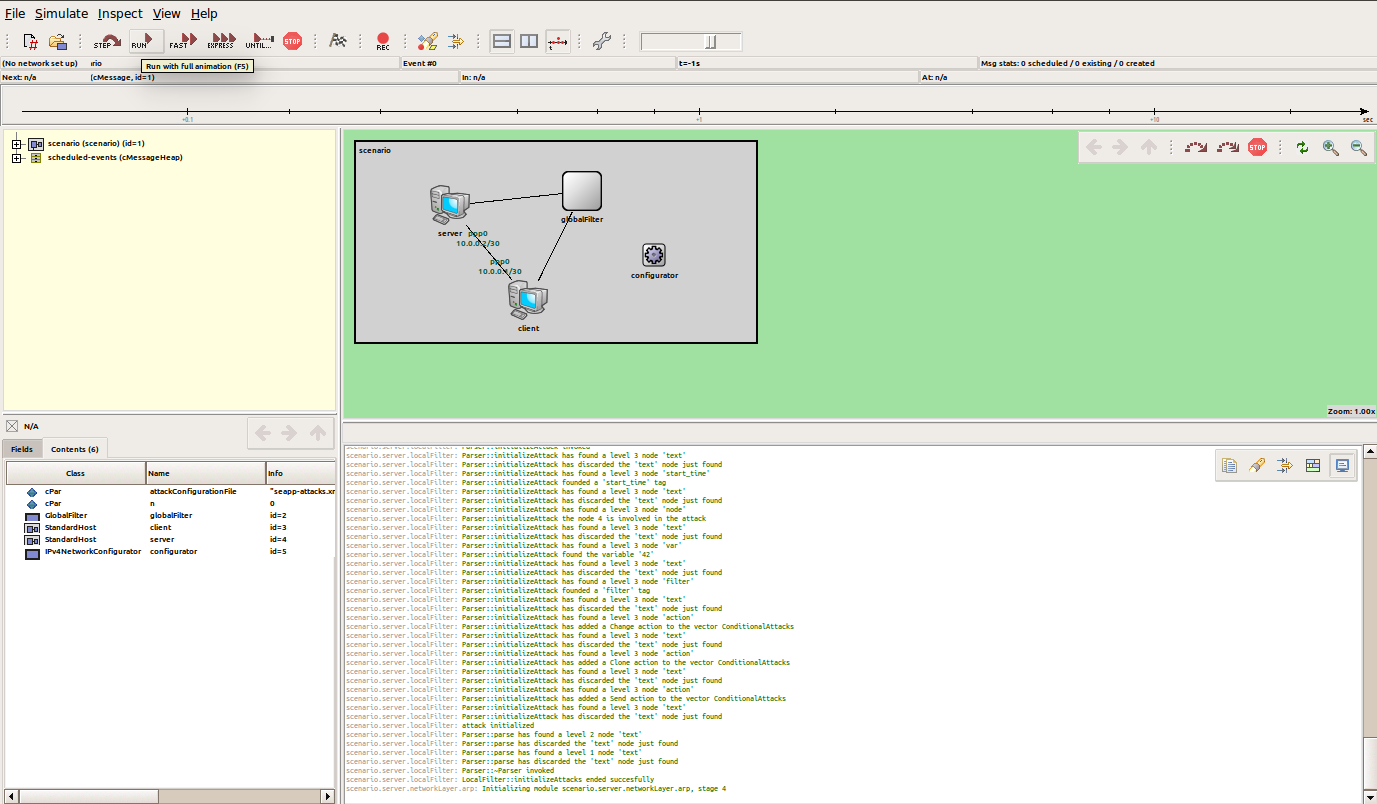
\includegraphics[width=.9\columnwidth]{appendix-scenario}
\caption{Simulation scenario}
\label{img:appendix-scenario}
\end{figure}
\end{landscape}


\section{SDN Architectures}
The same foundamental steps are followed in order to run an example in SDN architecture, with some small differences though. The main difference is that SDN nodes should be used. All the SDN-related nodes can be found under the \emph{/openflow} directory.

The below example shows a network with one client, one server, one OpenFlow switch and a SDN controller. The source code can be found under the \emph{/examples/inet\_sdn} direcory.

\paragraph{\nth{1} step - make the folder}
As in INET, the \nth{1} step is to make the folder that will contain all the new files, e.g. scenario.
%
\begin{lstlisting}[language={terminal}]
@~/seapp_stable/examples/inet_sdn@ mkdir scenario
@~/seapp_stable/examples/inet_sdn@ cd scenario
\end{lstlisting}


\paragraph{\nth{2} step - network description}
As in INET, the \nth{2} step is to edit the \texttt{.ned} file that contains the network description, e.g. \texttt{scenario.ned}.
%
\begin{lstlisting}[language={ned}, caption={scenario.ned}, label={lst:build-scenario-ned}]
package inet.examples.inet_sdn.scenario;

import inet.nodes.inet.StandardHost;
import inet.networklayer.autorouting.ipv4.FlatNetworkConfigurator;
import inet.util.ThruputMeteringChannel;

import inet.globalfilter.GlobalFilter;
import inet.exmachina.ExMachina;

import inet.openflow.nodes.*;

network Topo
{
    parameters:		
        string attackConfigurationFile = default("none");
		
    @display("bgb=2000,1000");
    types:
        channel ethernetline extends ThruputMeteringChannel {
            delay = 1us;
            datarate = 100Mbps;
        }
	submodules:
        configurator: FlatNetworkConfigurator {
            @display("p=1800, 500");
        }
        globalFilter: GlobalFilter {
            @display("p=1800,200");
        }
        exmachina: ExMachina {
        		@display("p=1800, 700");
        }
        client: StandardHost {
           @display("p=150,250;i=device/laptop");
        }
        server: StandardHost {
            @display("p=1500,350;i=device/server");
        }      
        open_flow_switch: Open_Flow_Switch_SEA  {
            @display("p=1000,650");
        }
        controller: Open_Flow_Controller_SEA {
            @display("p=1000,100");
        }

        
	connections allowunconnected:
        
        client.ethg++ <--> ethernetline <--> open_flow_switch.ethg++;
        server.ethg++ <--> ethernetline <--> open_flow_switch.ethg++;
        
        controller.ethg++ <--> ethernetline <--> open_flow_switch.gate_controller++;
        
        globalFilter.nodes++ <--> client.global_filter;
        globalFilter.nodes++ <--> server.global_filter;
        globalFilter.nodes++ <--> open_flow_switch.global_filter;
        globalFilter.nodes++ <--> controller.global_filter;			
}
\end{lstlisting}

In this step, is fundamental to:
%
\begin{itemize}
\item add the the string parameter \texttt{attackConfigurationFile} to the network;
\item import the GlobalFilter class, declare a GlobalFilter submodule and connect it to all the other nodes;
\item import the ExMachina class and declare an ExMachina submodule if \emph{disable} action is performed. The module does not need to be connected to the rest of the nodes;
\item import and declare an \textbf{Open\_Flow\_Switch\_SEA} submodule. This is the extended version of a simple open flow switch including SEA++ mechanism;
\item import and declare an \textbf{Open\_Flow\_Controller\_SEA} submodule. This is the extended version of SDN controller node including the SEA++ mechanism;
\item use the \emph{FlatNetworkConfigurator} to assign IP addresses to the nodes. The usage of IPv4NetworkConfigurator in SDN architectures is under development.
\end{itemize}

All the SDN-related components will be found under the \emph{/openflow} folder.
\paragraph{\nth{3} step - edit omnetpp.ini}
As in INET, the \nth{3} step is to edit the \texttt{omnetpp.ini} file. In this step is fundamental to bind the configuration(s) with the ACF(s), by overwriting the name of the network parameter \texttt{attackConfigurationFile} with the name of a particular ACF.
%
\begin{lstlisting}[language={ini}]
[General]
network = scenario
@sim-time-limit@  = 250s

// General settings 
// ...

// Config(s) specific settings

[Config simple_attack]
**.attackConfigurationFile = simple_attack.xml

[Config disable]
**.attackConfigurationFile = disable.xml

// ...
\end{lstlisting}

\paragraph{\nth{4} step - add the ACF}
The \nth{4} and last step is to add the ACF(s) in the folder.
Write the description of the attack in the \texttt{.adl} file. Compile the file using the \texttt{interpreter.py} in the \texttt{inet\_sdn/interpreter/interpreter} folder. The output will be the ACF file in \texttt{.xml} format.

%
\begin{lstlisting}[language={terminal}]
@~/seapp_stable/examples/inet_sdn/scenario@ ../../../interpreter/interpreter/interpreter.py -i simple_attack.adl -o simple_attack.xml
\end{lstlisting}
% 

\paragraph{Run the simulation}
The simulation is ready to run. In the terminal, run the bash script \texttt{run.sh} which calls \texttt{run\_inet} in the \texttt{src} folder:
%
\begin{lstlisting}[language={terminal}]
@~/seapp_stable/examples/inet_sdn/scenario@ ./run.sh
\end{lstlisting}
%
It will start the simulation supported by the GUI, as shown in figure ~\ref{img:scenario}.

To run the simulation in express mode without using the GUI, type the following by specifying the configuration:
\begin{lstlisting}[language={terminal}]
@~/seapp_stable/examples/inet_sdn/scenario@ ../../../src/run_inet -u Cmdenv -c general
\end{lstlisting}
%

or :
\begin{lstlisting}[language={terminal}]
@~/seapp_stable/examples/inet_sdn/scenario@ ../../../src/run_inet -u Cmdenv -c simple_attack
\end{lstlisting}
%

\begin{landscape}
\begin{figure}[b]
\centering
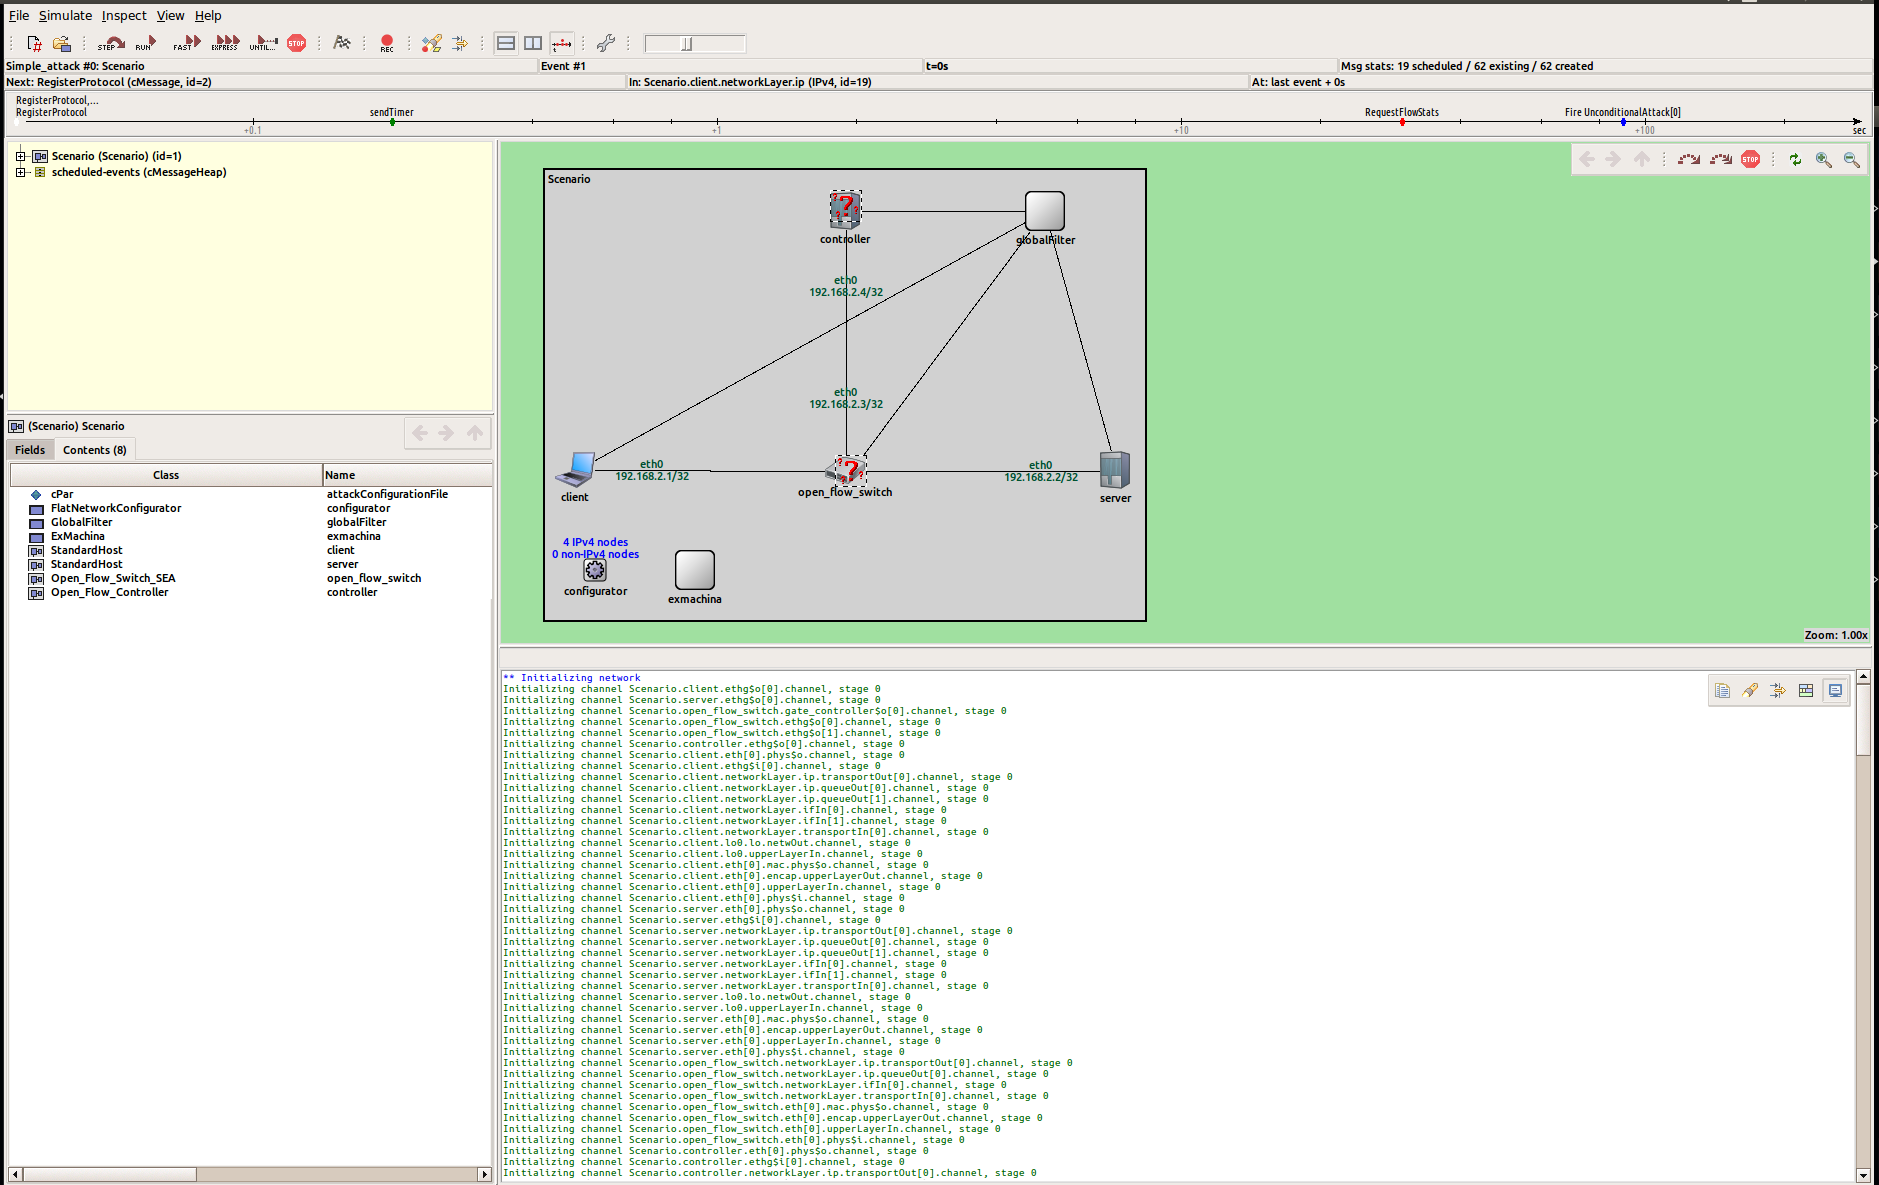
\includegraphics[width=.9\columnwidth]{sdn_scenario}
\caption{Simulation SDN scenario}
\label{img:scenario}
\end{figure}
\end{landscape}


 






